Experiments for LSH and CLSH are performed to evaluate their abilities in improving network inference algorithms' performance. We mainly focus on 3 existing algorithms: NetRate, ConNie , NetInf, on which we apply LSH and CLSH method respectively. 
%==========================
\subsection{Experiments on synthetic dataset}
Synthetic networks of 256 nodes are generated from Kronecker model with parameter matrix [0.5 0.5; 0.5 0.5]. At the beginning of each cascade, root node is selected randomly and recorded as $t=0$. Pairwise edge weights are sampled from $U(0,1)$. The larger the value of edge weight, the higher the probability of transmitting a message between this pair of nodes.  Once a node is infected, it begins to infect the adjacent nodes. Each activated node infects its neighbors with probabilities generated from transmission likelihood function( Exponential model). The diffusion proceeds iteratively until time window $T$, which is set at 10.
\\ Measures in this paper are AUC(Area under Precision-Recall curve) and maximum $F_1$ score. $F_1$ score is the harmonic mean of precision and recall while we consider the maximum value in evaluation.
\\ When generating synthetic cascade data, we use the piecewise function $S_p(t_j)$ to control life span heterogeneity. Value of $S_p(t_j)$ implies the diffusion speed of message in $t_j$. Large deviation in $S_p(t_j)$ causes strong heterogeneity. In this part, $S_p(t_j)$ is set as [0.03 0.9 0.07 0 0]. (time window $T=10$ as noted) When $T_j=3.2$, $S_p(t_j)=0.9$; when $T_j=5.9$, $S_p(t_j)=0.07$, etc.
\\\textbf{Performance vs. cascade number.} We make experiments of LSH-NetRate/LSH-ConNie/LSH-NetInf. By applying LSH method, the performance of network inference improves comparing with their original algorithms, as shown in Table \ref{tab:synLSHCASf1} and \ref{tab:synLSHCASAUC}. Figure \ref{fig:synLSHpr} plots the Precision-Recall curve of LSH-NetRate/LSH-ConNie/LSH-NetInf method. Our methods make distinct improvement.
\begin{table}[H]
\caption{Max $F_1$ score of LSH-NetRate/LSH-ConNie/LSH-NetInf vs. casNum}
\begin{tabular}{c|c|c|c}
 & casNum 300 & casNum 600 & casNum 900 \\
\hline
NetRate & 0.6742 & 0.7913 & 0.8161\\
LSH-NetRate & 0.7251 & 0.8210 & 0.8425\\
\hline
ConNie & 0.7500 & 0.7526 & 0.7905\\
LSH-ConNie & 0.7653 & 0.7734 & 0.8138\\
\hline
NetInf & 0.5927 & 0.6799 & 0.7360\\
LSH-NetInf & 0.6018 & 0.6997 & 0.7446
\end{tabular}\label{tab:synLSHCASf1}
\end{table}
%--------------
\begin{table}[H]
\caption{Area under PR curve of LSH-NetRate/LSH-ConNie/LSH-NetInf vs. casNum}
\begin{tabular}{c|c|c|c}
 & casNum 300 & casNum 600 & casNum 900 \\
\hline
NetRate & 0.4794 & 0.6299 & 0.6858\\
LSH-NetRate & 0.5573 & 0.6892 & 0.7805\\
\hline
ConNie & 0.6899 & 0.7424 & 0.7985\\
LSH-ConNie & 0.6916 & 0.7657 & 0.8334\\
\hline
NetInf & 0.3801 & 0.4638 & 0.5754\\
LSH-NetInf & 0.4186 & 0.5421 & 0.5764
\end{tabular}\label{tab:synLSHCASAUC}
\end{table}
\begin{figure*}
\centerline{
\subfigure[LSH-NetRate]{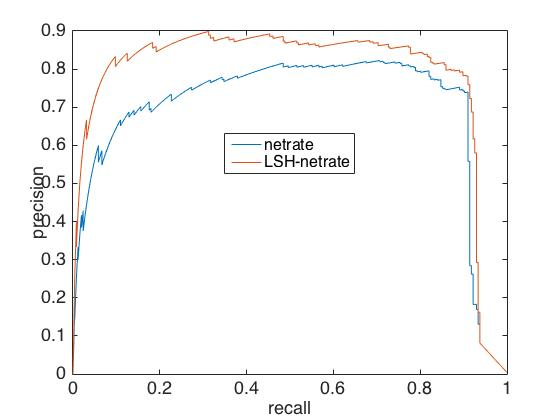
\includegraphics[width=0.35\linewidth]{figures/PR900.jpg}}
\subfigure[LSH-ConNie]{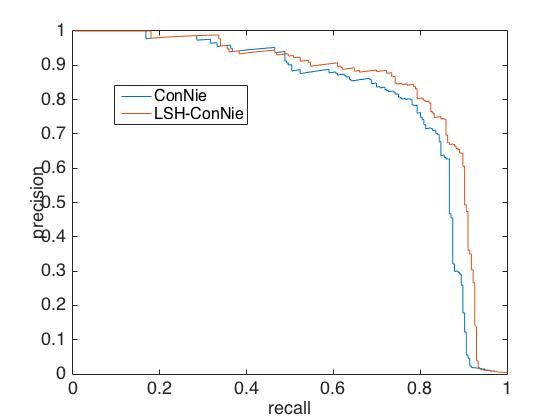
\includegraphics[width=0.35\linewidth]{figures/Connie900.jpg}}
\subfigure[LSH-NetInf]{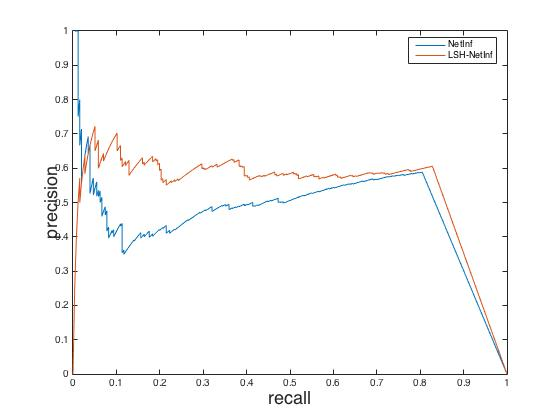
\includegraphics[width=0.35\linewidth]{figures/NetInfPR.jpg}}}
\caption{Precision-Recall curve of LSH-NetRate/LSH-ConNie/LSH-NetInf method }\label{fig:synLSHpr}
\end{figure*}
%--------------
\textbf{Performance vs. heterogeneity strength.} We generate synthetic cascades with various heterogeneity strength, as shown in Table \ref{tab:Spfunction}. The level of standard deviation depicts the strength of heterogeneity. Experiments in Figure \ref{fig:Hete} show that our method gains larger advantage to original NetRate as standard deviation of $S_p$ increases.
\begin{table}[H]
\caption{4 types of Sp function with different standard deviation.}
\begin{tabular}{c|c|c}
 & Sp function & standard deviation \\
\hline
1 & [0.2 0.2 0.2 0.2 0.2] & 0\\
2 & [0.2 0.4 0.3 0.05 0.05] & 0.1541\\
3 & [0.1 0.6 0.3 0 0] & 0.2549\\
4 & [0.03 0.9 0.07 0 0] & 0.3924
\end{tabular}\label{tab:Spfunction}
\end{table}
\begin{figure}[H]
\centerline{
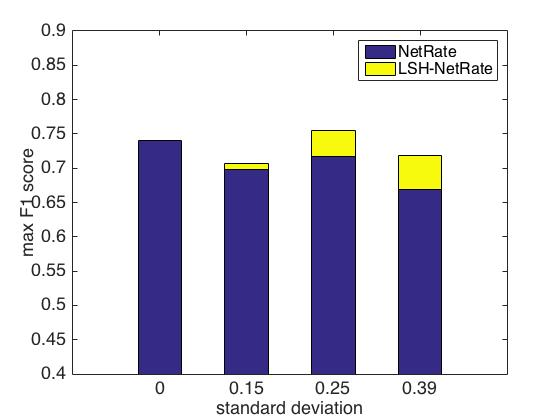
\includegraphics[width=0.75\linewidth]{figures/HeteroStrength.jpg}}
\caption{Experiments on different heterogeneity strength. }\label{fig:Hete}
\end{figure}
%--------------
\textbf{Setting of $lag$.} $lag$ is half the length of sliding window around target time stamp that can affect the estimation of $S_p$. We run our methods with 4 different $lag$ settings separately, results are shown in Figure \ref{fig:SetLAG}. We can see that their differences are slight as we change $lag$'s value. But LSH method performs better with $lag$ set around 10\% of T.
\begin{figure}[H]
\centerline{
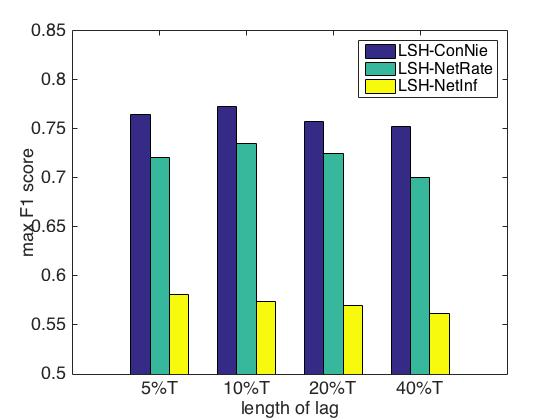
\includegraphics[width=0.75\linewidth]{figures/SettingLAG.jpg}}
\caption{Experiments of different lag values. }\label{fig:SetLAG}
\end{figure}
%--------------
\textbf{Experiments of CLSH method.}
CLSH method attempts to cluster cascades so that cascades in the same group have similar $S_p(t_j)$. In this part, we use 3 types of $S_p(t_j)$ functions: [0.1 0.8 0.1 0 0] / [0.8 0.2 0 0 0] / [0 0 0 0.2 0.8]. Before simulating a cascade, we randomly choose one of this three to be the specific $S_p$ function of this cascade.  
\\\textbf{Performance of CLSH vs. cascade number.} We make experiments of CLSH-NetRate/CLSH-ConNie/CLSH-NetInf methods on synthetic cascades with multiply heterogeneity functions. As shown in Table \ref{tab:synCLSHCASf1} and \ref{tab:synCLSHCASAUC}, our methods outperform the original algorithms on max $F_1$ score and $AUC$. 
\begin{table}[H]
\caption{Max $F_1$ score of CLSH-NetRate/CLSH-ConNie/CLSH-NetInf vs. casNum}
\begin{tabular}{c|c|c|c}
 & casNum 300 & casNum 600 & casNum 900 \\
\hline
NetRate & 0.7124 & 0.7222 & 0.7254\\
CLSH-NetRate & 0.7256 & 0.7425 & 0.7414\\
\hline
ConNie & 0.7296 & 0.7531 & 0.7619\\
CLSH-ConNie & 0.7474 & 0.7520 & 0.7692\\
\hline
NetInf & 0.6727 & 0.7133 & 0.7316\\
CLSH-NetInf & 0.6886 & 0.7314 & 0.7489
\end{tabular}\label{tab:synCLSHCASf1}
\end{table}
%---------------
\begin{table}[H]
\caption{Area under PR curve of CLSH-NetRate/CLSH-ConNie/CLSH-NetInf vs. casNum}
\begin{tabular}{c|c|c|c}
 & casNum 300 & casNum 600 & casNum 900 \\
\hline
NetRate & 0.5243 & 0.5445 & 0.5894\\
CLSH-NetRate & 0.5771 & 0.6527 & 0.6582\\
\hline
ConNie & 0.7006 & 0.7449 & 0.7612\\
CLSH-ConNie & 0.7194 & 0.7600 & 0.7602\\
\hline
NetInf & 0.4079 & 0.4248 & 0.5138\\
CLSH-NetInf & 0.4319 & 0.4402 & 0.5268
\end{tabular}\label{tab:synCLSHCASAUC}
\end{table}
\textbf{Setting of $k$.} As shown in Figure \ref{fig:SetK}, clustering cascades into 3 $\sim$ 4 groups produces higher accuracy.
\begin{figure}[H]
\centerline{
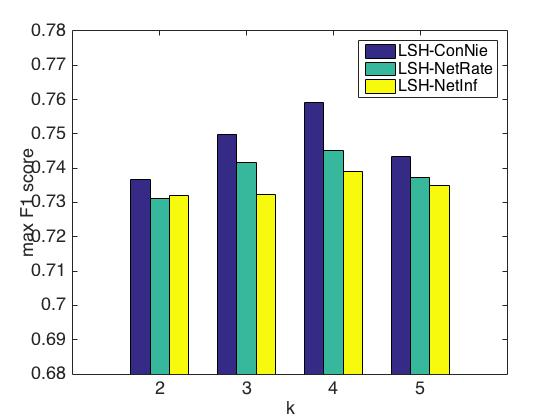
\includegraphics[width=0.75\linewidth]{figures/SettingK.jpg}}
\caption{Experiments of different k values. }\label{fig:SetK}
\end{figure}
%==========================
\subsection{Experiments on real world dataset}
We use \emph{U.S. patent dataset} by \emph{the National Bureau of Economic Research} to test (C)LSH method. The dataset spans 25 years from 1975 to 1999, containing 16,522,438 citations. Inventors of patents cite their sources. Therefore, we take inventors as the entities of network and follow the citations to reveal information flow. Note that we remove all self-loops in patent data, which happen when inventors cite their own previous works. By ranking inventors according to their activity, we have 147 most active inventors to form the ground truth network. We extract 150/250/350/450 transmission trees for cascade information. Experiments of (C)LSH-NetRate, (C)LSH-ConNie, (C)LSH-NetInf are made on this dataset. 
\\For real world dataset, the lengths of cascades differ a lot. We apply Min-Max Normalization to activation times in each cascade separately. Cascades' length is 1 after transformation.
\begin{itemize}
\item (C)LSH-NetRate
\\ \textbf{Performance vs. cascade number. }From Table \ref{tab:rwdLSHnetrateCASf1} we can see improvement by applying LSH method to NetRate on various data scale. Increasing $k$ in some occasions can help improve accuracy.
\begin{table}[H]
\caption{Real data: Max $F_1$ score of NetRate/  LSH-NetRate/ CLSH-NetRate vs. casNum}
\begin{tabular}{c|c|c|c|c}
 & cas 150 & cas 250 & cas 350 & cas 450 \\
 \hline
 NetRate & 0.5915 & 0.6110 & 0.6418 & 0.6667 \\
 LSH-NetRate & 0.6324 & 0.6364 & 0.6817 & 0.6975 \\
 CLSH-k 3 & 0.6328 & 0.6431 & 0.6731 & 0.6997 \\
 CLSH-k 5 & 0.6324 & 0.6360 & 0.6752 & 0.7121
\end{tabular}\label{tab:rwdLSHnetrateCASf1}
\end{table}
%--------------
\item (C)LSH-ConNie
\\ \textbf{Performance vs. cascade number.} LSH method outperforms ConNie notably as shown in Table \ref{tab:rwdLSHconnieCASf1}. Furthermore, applying CLSH to cluster similar cascades extends the performance advantage over original ConNie method.
\begin{table}[H]
\caption{Real data: Max $F_1$ score of ConNie/  LSH-ConNie/ CLSH-ConNie vs. casNum}
\begin{tabular}{c|c|c|c|c}
 & cas 150 & cas 250 & cas 350 & cas 450 \\
 \hline
 ConNie & 0.5702 & 0.6127 & 0.6412 & 0.6788 \\
 LSH-ConNie & 0.8125 & 0.8222 & 0.8532 & 0.8673 \\
 CLSH-k 3 & 0.8249 & 0.8298 & 0.8502 & 0.8733 \\
 CLSH-k 5 & 0.8140 & 0.8218 & 0.8561 & 0.8581
\end{tabular}\label{tab:rwdLSHconnieCASf1}
\end{table}
%--------------
\item (C)LSH-NetInf
\\ \textbf{Performance vs. cascade number.} Table \ref{tab:rwdLSHnetinfCASf1} and \ref{tab:rwdLSHnetinfCASauc} present the AUC and maximum $F_1$ score results of our methods and NetInf algorithm. In all cases, our methods perform better than NetInf. When including more cascades, the complexity increases. Proper increment of $k$ may lead to higher performance.
\begin{table}[H]
\caption{Real data: Max $F_1$ score of NetInf/  LSH-NetInf/ CLSH-NetInf vs. casNum}
\begin{tabular}{c|c|c|c|c}
 & cas 150 & cas 250 & cas 350 & cas 450 \\
 \hline
 NetInf & 0.5284 & 0.5382 & 0.5779 & 0.5981 \\
 LSH-NetInf & 0.7604 & 0.7762 & 0.7993 & 0.7932 \\
 CLSH-k 3 & 0.7757 & 0.7902 & 0.8000 & 0.7938 \\
 CLSH-k 5 & 0.7833 & 0.7762 & 0.8129 & 0.8062
\end{tabular}\label{tab:rwdLSHnetinfCASf1}
\end{table}
\begin{table}[H]
\caption{Real data: AUC of NetInf/ LSH-NetInf/ CLSH-NetInf vs. casNum}
\begin{tabular}{c|c|c|c|c}
 & cas 150 & cas 250 & cas 350 & cas 450 \\
 \hline
 NetInf & 0.7860 & 0.7919 & 0.8160 & 0.8292 \\
 LSH-NetInf & 0.9413 & 0.9393 & 0.9410 & 0.9429 \\
 CLSH-k 3 & 0.9502 & 0.9473 & 0.9418 & 0.9436 \\
 CLSH-k 5 & 0.9547 & 0.9393 & 0.9490 & 0.9506
\end{tabular}\label{tab:rwdLSHnetinfCASauc}
\end{table}
\end{itemize}